\subsection{Pearson Correlation}\label{subsec:pearsoncorrelation}

In order to test the validity of our metrics and the chosen policy, a the pearson correlation between the metrics have been conducted. The point of the test is to make sure no metrics are directly correlating, meaning one of the metrics is negligible. There is a number of different reasons as to why the outcome will look as it does, and it will be discussed thoroughly. The Pearson-Correlation have been calculated on the individual scores given to a trip per each of metrics. 

The matrix of pearson correlations between the metrics is shown at table \ref{tab:pearsonmatrix}. The most notable result is the multicollinearity between accelerations and brakes, which seems rather odd as they are diametrical opposites and can per definition not exist at the same time. Another highly correlating metric is jerks having a correlation of 0.828 with both brakes and accelerations. 

\begin{table*}[tb]
\centering
\caption{This is the pearson correlation matrix between the metrics}
\label{tab:pearsonmatrix}
\begin{tabular}{l|llllll}
                      & Roadtypes & Critical Time Periods & Speeding & Accelerations & Brakes & Jerks  \\ \hline
Roadtypes             & 1         & -0.250                & -0,546   & -0.341        & -0,348 & -0,241 \\
Critical Time Periods & -0.250    & 1                     & 0.156    & 0.460         & 0.428  & 0.313  \\
Speeding              & -0,546    & 0.156                 & 1        & 0.196         & 0.195  & 0.144  \\
Accelerations         & -0.341    & 0.460                 & 0.196    & 1             & 0.971  & 0.828  \\
Brakes                & -0,348    & 0.428                 & 0.195    & 0.971         & 1      & 0.828  \\
Jerks                 & -0,241    & 0.313                 & 0.144    & 0.828         & 0.828  & 1     
\end{tabular}
\end{table*}

Looking closer at the multicollinearity between accelerations and brakes, there is a couple of different factors which affect the result. As mentioned accelerating and braking are diametrically opposite, but they are both dependant of the speed of the vehicle (as they are calculated through the change in speed). If the driver performs a big acceleration, his speed is high and he at some point needs to brake in order to decline in speed. 

\begin{figure}[tb]
\centering
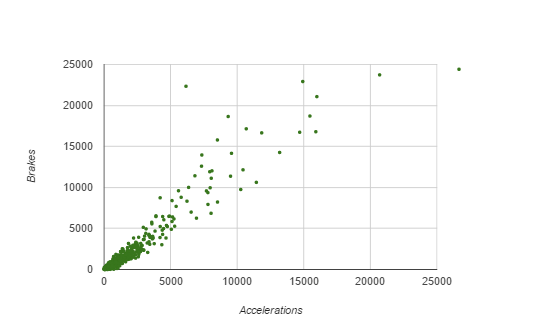
\includegraphics[width=0.465\textwidth]{Pictures/abcorrel}
\caption{The correlation between accelerations and brakes}
\label{fig:abcorrel}
\end{figure}

The figure shown at \ref{fig:abcorrel} clearly illustrates the correlation. Another reasoning as to why these metrics correlate can be the thresholds in the policy used to calculate the scores. As earlier mentioned the threshold for brakes are 8 $m/s^2$ whereas accelerations are counted from 5 $m/s^2$. If we had no thresholds and the delinquencies were scored the same, the correlation would be 1.0 as it only depended on the speed of the vehicle. 
Jerks was the metric met with the highest level of scepticism when implemented, and the correlation shows that it was not completely unwarranted. It does show a lot of correlation with both brakes and accelerations. The figure \ref{fig:ajcorrel} shows the correlation between accelerations and jerks. Jerks are as mentioned calculated as $m/s^3$, and a driver with many accelerations are almost bound to have a lot of jerks as it is hard to keep a constant acceleration.

\begin{figure}[tb]
\centering
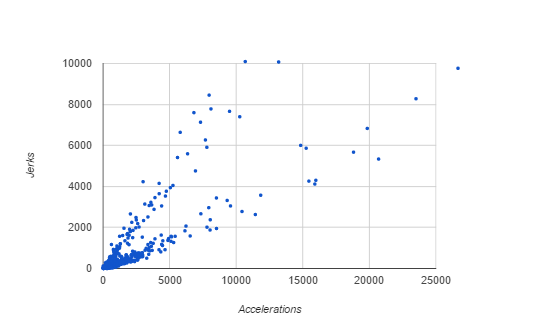
\includegraphics[width=0.465\textwidth]{Pictures/ajcorrel}
\caption{The correlation between accelerations and jerks}
\label{fig:ajcorrel}
\end{figure}


the similar correlation between the two can be answered by the correlation between accelerations and brakes. 

